\documentclass{article}
\usepackage[utf8]{inputenc}
\title{Vioeo 4: Confidence Intervals}
\author{wbg231 }
\date{December 2022}
\newcommand{\R}{$\mathbb{R}$}
\newcommand{\B}{$\beta$}
\newcommand{\A}{$\alpha$}
\newcommand{\D}{\Delta}
\newcommand{\avector}[2]{(#1_2,\ldots,#1_{#2})}
\newcommand{\makedef}[2]{$\textbf{#1}$:#2 }
\usepackage{tikz,graphicx,hyperref,amsmath,amsfonts,amscd,amssymb,bm,cite,epsfig,epsf,url}

\begin{document}

\maketitle

\section{plan}
\begin{itemize}
\item \href{https://www.youtube.com/watch?v=soWJ3Wti0FM}{video link}
\item intuit on 
\item definition
\item interpretation
\section{intuition}
\subsection{estimation of population parameter}
\item we want to estimate some population parameter for a very large population, so we have to use a subset of the population 
\item a simple idea is to chose a random subset of the population that is iid. 
\subsection{random sampling}
\item random sampling does really well with the population mean and population proportion 
\item every time we take random samples our estimate of population parameter changes.
\item so our estimate of the population parameter is a random variable and thus has uncertainty
\item so our goal is to try to characterize our uncertainty about the estimator from the data we have available (ie the sample )
\section{confidence interval}
\subsection{confidence intervals}
\item the main idea is to report a range of values that contain the parameter with a high probability (which is typically 95 percent)
\item so lets try to build a confidence interval for the population mean
\subsection{sample mean}
\item the population population mean is $\mu_{pop}$ and population variance is $\sigma_{pop}^{2}$
\item random samples are selected independently and uniformly at random with replacement $\Tilde{x}_1...\Tilde{x}_n$ from the population. 
\item the sample mean $\Tilde{m}=\frac{1}{n}\Sigma_{i=1}^{n}\Tilde{x}_{i}$
\item $E[m]=\mu$ and sample mean is unbiased
\item $se(m)=\frac{\sigma}{\sqrt{n}}$ that is the standard error of the sample mean is decreasing in n 
\item further we know that as $n\rightarrow \infty$ $\Tilde{m}_{n}$ converges in distribution to a Gaussian with mean $\mu_{pop}$ and variance $se(\Tilde{m}))=\frac{1\sigma}{\sqrt{n}}$
\item so in other words we know the distribution of our sample means will look like this 
\item 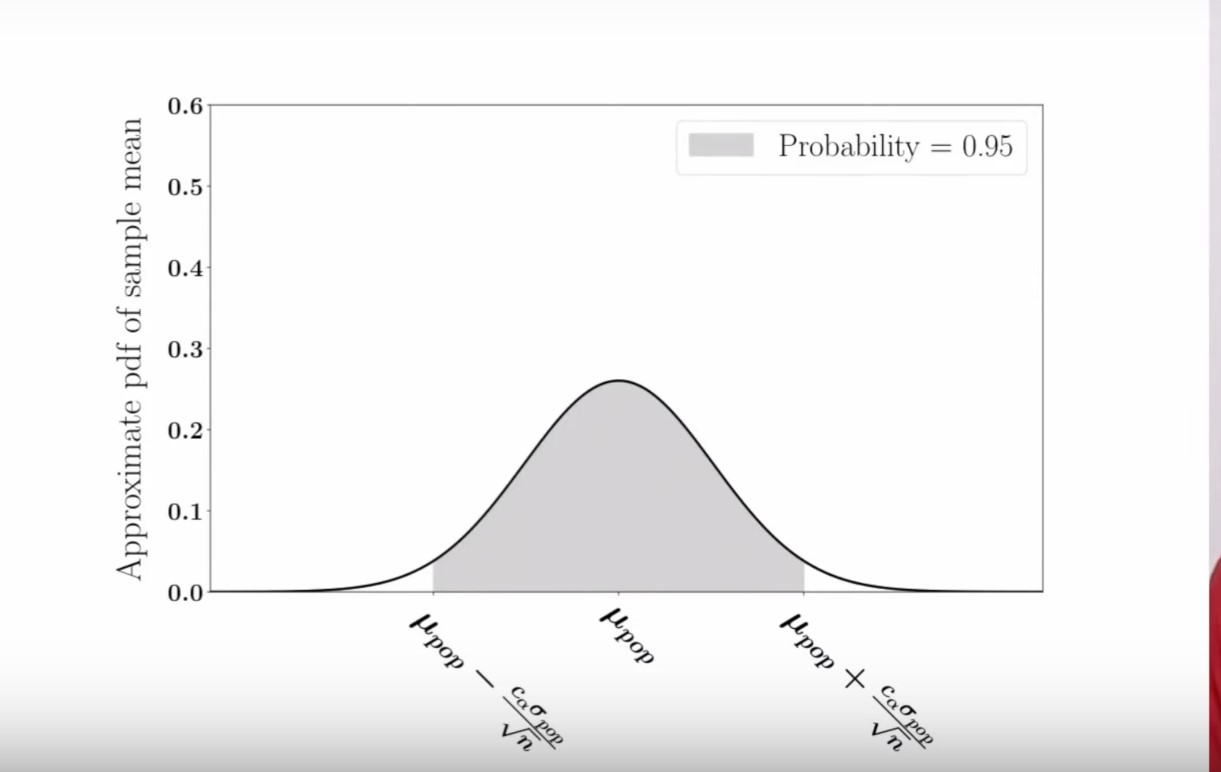
\includegraphics[width=10cm]{notes/week_4/vidio 4: Confidince Intervals/immages/v4_1.jpg}
\item so it is easy to build an interval that contains the sample mean with a certain probability.
\item so this is the likely hood that any given sample of size n will be there 
\item $\Tilde{m}\in [\mu_{pop}-c,\mu_{pop}+c]$ for some number c. is this a confidence interval? 
\item no because we are constructing this based off $\mu_{pop}$ which we do not have 
\item but if this is true  $\Tilde{m}\in [\mu_{pop}-c,\mu_{pop}+c]$ we can write $\mu_{pop}-c\leq \Tilde{m}\leq \mu_{pop}+c$ this gives us $\mu-c\leq m\Rightarrow \mu\leq m+c$ as well as $\mu+c\geq m\Rightarrow \mu\geq m-c$ thus we have  $\mu_{pop}\in [\Tilde{m}-c, \Tilde{m}+c]$
\item so now we have a confidince interval that depends on the sample mean which is what we compute from the data, then we can find some c to establish the width of the interval such that $\mu_{pop}\in [\Tilde{m}-c, \Tilde{m}+c]$ will happen with a certain likelihood
\item which is what we wanted 
\item so if we get a sample mean from n measurements that is red line x. we know the likelihood it is in the shaded area is 95 percent   
\item 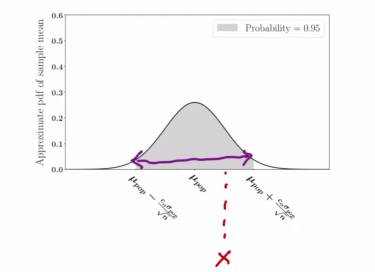
\includegraphics[width=10cm]{notes/week_4/vidio 4: Confidince Intervals/immages/v4_2.jpg}
\item this implies that if have an interval of the same length as the shaded area centered at the sample mean, then that interval has a 95 percent chance of containing the population mean 
\item so now every time we obtain a sample mean as long as we know the width of this interval we can build a confidence interval. 
\item 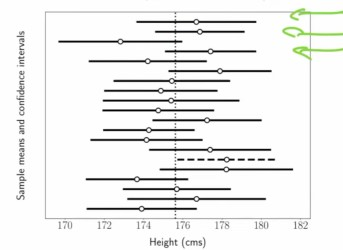
\includegraphics[width=10cm]{notes/week_4/vidio 4: Confidince Intervals/immages/v4_3.jpg}
\item so this image shows the confidence intervals obtained from many different samples and there sample means 
\item an notice that much of the time this confidence interval does indeed capture the population parameter 
\subsection{shifting Gaussian}
\item remember that if $\Tilde{a}$ is Gaussian with $\mu, \sigma^{2}$ ie $\Tilde{a}\sim \mathcal{N}(\mu,\sigma^2)$
\item then $\Tilde{b}=\alpha \Tilde{a}+\beta$ will be $\Tilde{b}\sim \mathcal{N}(\alpha \mu+\beta, \alpha^2\sigma^2 )$
\subsection{confidence interval for a Gaussian }
\item suppose we have $\Tilde{a}$ such that $\Tilde{a}\sim \mathcal{N}(\mu,\sigma^2)$ which we are using to estimate some true quantity  $A$
\item so we can define an interval that has a $(1-\alpha)$ percent chance to contain A as $\Tilde{\mathcal{I}}_{1-\alpha}=[\Tilde{a}-c_{\alpha}\sigma,\Tilde{a}+c_{\alpha}\sigma]$ 
\item where $c_{\alpha}$ is  is some constant determined by $1-\alpha$ which is the likelihood that that interval contains a 
\item so the interval is centred at a and the width is determined by the standard deviation ie $\sigma$
\item keep in mind $\Tilde{\mathcal{I}}_{1-\alpha}$ that is the interval is random, A that is what we are trying to estimate is fixed
\item so how can we chose $c_{\alpha}$ such that the $P(A\in\Tilde{\mathcal{I}}_{1-\alpha})=(1-\alpha) $?
\item we lets look at this $P(A\in \Tilde{\mathcal{I}}_{1-\alpha})=1-P(\Tilde{a}-c_{\alpha}>A)- P(\Tilde{a}+c_{\alpha}<A)$ that is 1 minus the probability of the likelihood it is not in that interval which are two disjoint events 
\item $P(A\in \Tilde{\mathcal{I}}_{1-\alpha})=1-P(\Tilde{a}-c_{\alpha}>A)- P(\Tilde{a}+c_{\alpha}<A)=1-P(\frac{a-\mu}{\sigma}>c_{\alpha})-P(\frac{a-\mu}{\sigma}<-c_{\alpha})$ call $\Tilde{z}\sim \mathcal{N}(0,1)$ the standardized version of $\Tilde{a}$
\item $P(A\in \Tilde{\mathcal{I}}_{1-\alpha})=1-P(\Tilde{a}-c_{\alpha}>A)- P(\Tilde{a}+c_{\alpha}<A)=1-P(\frac{a-\mu}{\sigma}>c_{\alpha})-P(\frac{a-\mu}{\sigma}<-c_{\alpha})=1-p(\Tilde{z}>c_{\alpha})-p(\Tilde{z}<-c_{\alpha})$ by symmetry this is $P(A\in \Tilde{\mathcal{I}}_{1-\alpha})=1-P(\Tilde{a}-c_{\alpha}>A)- P(\Tilde{a}+c_{\alpha}<A)=1-P(\frac{a-\mu}{\sigma}>c_{\alpha})-P(\frac{a-\mu}{\sigma}<-c_{\alpha})=1-p(\Tilde{z}>c_{\alpha})-p(\Tilde{z}<-c_{\alpha})=1-2P(\Tilde{z}>c_{\alpha})$ this we can just compute 
\item so that is the value that if we plug into a normal rv will ensure it will capture 1-alpha percentage of the time 
\item we can write $c_{\alpha}=F_\Tilde{z}^{-1}(1-\frac{\alpha}{2})$ so we can calculate this value for any $1-\alpha$ value we want 
\item so if we know $\sigma^2$ that is the variance of our Gaussian $\Tilde{a}$ we can compute $c_{\alpha}$ such that $P(A\in \Tilde{\mathcal{I}}_{1-\alpha})=1-\alpha$
\subsection{confidence interval for the population mean }
\item the population population mean is $\mu_{pop}$ and population variance is $\sigma_{pop}^{2}$
\item random samples are selected independently and uniformly at random with replacement $\Tilde{x}_1...\Tilde{x}_n$ from the population. 
\item the sample mean $\Tilde{m}=\frac{1}{n}\Sigma_{i=1}^{n}\Tilde{x}_{i}$
\item $E[m]=\mu$ and sample mean is unbiased
\item $se(m)=\frac{\sigma}{\sqrt{n}}$ that is the standard error of the sample mean is decreasing in n 
\item further we know that as $n\rightarrow \infty$ $\Tilde{m}_{n}$ converges in distribution to a Gaussian with mean $\mu_{pop}$ and variance $se(\Tilde{m}))=\frac{1\sigma}{\sqrt{n}}$
\item so then assuming that the sample mean is Gaussian which holds for really large values of n we can write $\Tilde{\mathcal{I}}_{1-\alpha}=[\Tilde{m}-c_{\alpha}se(m),\Tilde{m}+c_{\alpha}se(m)]=[\Tilde{m}-\frac{c_{\alpha}\sigma_{pop}}{\sqrt{n}},\Tilde{m}+\frac{c_{\alpha}\sigma_{pop}}{\sqrt{n}}]$ where  $c_{\alpha}=F_\Tilde{z}^{-1}(1-\frac{\alpha}{2})$
\item the issue with this is we don't know $\sigma_{pop}$
\subsection{so what now?}
\item we don't know $\sigma_{pop}$ so we can just use the sample standard deviation or use an upper bound 
\item we can use the sample standard deviation as we know it is a consistent unbiased estimator of the population standard deviation and thus is likely to give a reasonable estimate 
\section{interpretation}
\subsection{logic}
\item so we are saying that if we assume our estimator is distributed as a Gaussian rv, 
\item we can use 1 sample to estimate the estimator, construct a confidence interval centred at the estimator and has a 1-alpha chance of having the population parameter 
\item so that is how we can build these confidence intervals
\item 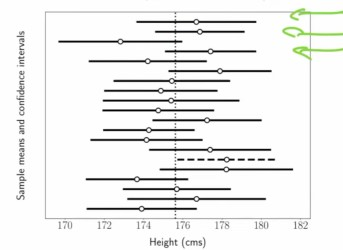
\includegraphics[width=10cm]{notes/week_4/vidio 4: Confidince Intervals/immages/v4_3.jpg}
\item notice the width of the confidence interval is determined by n. so a small n means a large width 
\item as we increase n the confidence intervals will get more narrow, but we are holding the likelihood that they contain the estimator set at $\1-\alpha$ percent
\item this means that there is a $\alpha$ percent chance that our interval does not have the parameter
\item we have less uncertainty about our estimate as n grows
\subsection{interpretation}
\item suppose we have a .95 percent certain confidence interval for the population mean of height data as [175,178]
\item \textbf{we can not say} the probability the population mean is in the interval is in that range, since the population mean is fixed our estimator is uncertain 
\item \textbf{we can say} if we were to repeat our measurement process many times. 95 percent of the time our interval will contain the populating mean 
\item  \textbf{we can say} if we build many .95\% confidence intervals 95\% of them contain the population mean 
\item  \textbf{we can say} 95\% of the time our interval will contain the fixed population parameter

\end{itemize}
\end{document}
